% =====================================================================
%  Bitcoin Wallet Risk Analyzer — Project Book (Data-Science Project)
%  Seminar Projects, 2025-2026 (Tashpah)
%  COMPILE WITH XeLaTeX (needed for the Hebrew abstract).
%    latexmk -xelatex main.tex
%  or:  xelatex -> bibtex -> xelatex -> xelatex
% =====================================================================
\documentclass[12pt,a4paper,openany]{report}

% ---------- Geometry & spacing ----------
\usepackage[a4paper,top=1in,bottom=1in,left=1.1in,right=1in]{geometry}
\usepackage{setspace}
\onehalfspacing                 % 1.5 line spacing (course requirement)

% ---------- Fonts / languages (XeLaTeX) ----------
\usepackage{fontspec}
\setmainfont{Liberation Serif}
\setsansfont{Liberation Sans}
\setmonofont{Liberation Mono}

% Hebrew (abstract) via XeTeX native RTL — avoids the bidi dependency.
\newfontfamily\hebrewfont[Script=Hebrew]{DejaVu Sans}
\TeXXeTstate=1
\newcommand{\heb}[1]{{\hebrewfont\beginR #1\endR}}
\newcommand{\hebpar}[1]{{\raggedleft\hebrewfont\beginR #1\endR\par}}

% ---------- Core packages ----------
\usepackage{microtype}
\usepackage{graphicx}
\usepackage{booktabs}
\usepackage{array}
\usepackage{tabularx}
\usepackage{multirow}
\usepackage{amsmath}
\usepackage{amssymb}
\usepackage{enumitem}
\usepackage{xcolor}
\usepackage{caption}
\usepackage{float}
\usepackage[numbers,sort&compress]{natbib}
\usepackage{titlesec}
\usepackage[hidelinks,breaklinks]{hyperref}

\definecolor{accent}{HTML}{2563EB}
\definecolor{ink}{HTML}{1E293B}
\hypersetup{colorlinks=true,linkcolor=accent,citecolor=accent,urlcolor=accent}

\captionsetup{font=small,labelfont=bf,labelsep=period}
\newcolumntype{Y}{>{\raggedright\arraybackslash}X}
\newcolumntype{C}{>{\centering\arraybackslash}X}
\setlength{\emergencystretch}{3em}

% ---------- Chapter/section title styling (compact) ----------
\titleformat{\chapter}[hang]{\LARGE\bfseries\color{ink}}{\thechapter.}{0.5em}{}
\titlespacing*{\chapter}{0pt}{6pt}{14pt}
\titleformat{\section}{\large\bfseries\color{ink}}{\thesection}{0.6em}{}
\titleformat{\subsection}{\normalsize\bfseries\color{ink}}{\thesubsection}{0.5em}{}

% Every chapter starts at the top of a new page (report-class default with
% openany), so a chapter heading never appears in the middle of a page.
\usepackage{etoolbox}

\newcommand{\repo}{\href{https://github.com/NehorayChalfon0166/final_project}{github.com/NehorayChalfon0166/final\_project}}
\newcommand{\live}{\href{https://cryptotrace.cs.bgu.ac.il/}{cryptotrace.cs.bgu.ac.il}}

% =====================================================================
\begin{document}
\sloppy

% ===================== TITLE PAGE ====================================
\begin{titlepage}
\centering
\vspace*{0.6cm}
{\large Ben-Gurion University of the Negev\par}
{\large Faculty of Natural Sciences\par}
{\large Department of Computer Science\par}
\vspace{1.6cm}

\rule{\linewidth}{0.4pt}\\[0.5cm]
{\Huge\bfseries Bitcoin Wallet Risk Analyzer\par}
\vspace{0.35cm}
{\large Detecting Criminal Bitcoin Wallets with Graph Neural Networks\par}
\vspace{0.35cm}
{\large\itshape \heb{מנתח סיכון לארנקי ביטקוין — זיהוי ארנקים פליליים באמצעות רשתות נוירונים גרפיות}\par}
\rule{\linewidth}{0.4pt}\\[1.4cm]

{\large\bfseries Project Team\par}
\vspace{0.3cm}
{\large
Ori Sinvani \quad(325770824)\\[3pt]
Harel Brener \quad(214179012)\\[3pt]
Nehoray Chalfon \quad(325833531)\par}
\vspace{1.1cm}

{\large\bfseries Project Advisor\par}
\vspace{0.2cm}
{\large Ofer Zevin\par}
\vfill

{\large Project Year: 2025--2026 \; (\heb{תשפ"ו})\par}
\vspace{0.5cm}
{\small Code repository: \repo\\ Live demo: \live}
\end{titlepage}

% ===================== ABSTRACTS ====================================
\pagenumbering{roman}
\setcounter{page}{2}

\chapter*{Abstract}
\addcontentsline{toc}{chapter}{Abstract}
Cryptocurrency networks are increasingly exploited for money laundering, ransomware
payments, fraud, and terror financing. Because Bitcoin is pseudonymous and its transaction
graph is massive and dynamic, the compliance teams at banks, exchanges, and
law-enforcement agencies still rely mostly on static blacklists that only flag wallets
\emph{after} they are already known to be malicious. This project asks a data-science
question instead: given only a Bitcoin address and its public transaction history, can we
decide whether the wallet has been used for criminal activity?

We frame the problem as binary node classification over per-wallet ego-graphs and train a
three-layer \textbf{GATv2} graph attention network that reads both a wallet's own behaviour
and the pattern of its one-hop transactions. The model is trained on a balanced merge of two
public labelled datasets, \textbf{REAL-CATS} (modern criminal wallets) and
\textbf{Elliptic++} (theft/Ponzi era), comprising 86{,}870 training wallets and 21{,}718
held-out test wallets. On the held-out test set the GNN reaches an \textbf{F\textsubscript{1}
of 0.869}, accuracy 0.894, recall 0.884, and \textbf{ROC-AUC 0.959}, with well-calibrated
probabilities after temperature scaling. It beats an XGBoost classifier trained on the same
twelve tabular features (F\textsubscript{1} 0.755) and a plain GCN baseline
(F\textsubscript{1} 0.582). The $\sim$11-point F\textsubscript{1} gap over XGBoost is the
central finding: the local transaction structure around a wallet carries information that the
wallet's own summary statistics do not. The trained model is served through a FastAPI backend
and a React web application deployed at \live.

% ----- Hebrew abstract (RTL, native XeTeX) — follows the English one -----
\vspace{1.4em}
{\noindent\LARGE\bfseries\heb{תקציר}\par}
\addcontentsline{toc}{chapter}{\heb{תקציר} (Hebrew Abstract)}
\vspace{0.5em}
\hebpar{רשתות מטבעות קריפטוגרפיים מנוצלות יותר ויותר להלבנת הון, תשלומי כופרה, הונאה ומימון טרור. מכיוון שביטקוין הוא פסאודו-אנונימי וגרף העסקאות שלו עצום ודינמי, צוותי הרגולציה בבנקים, בבורסות ובגופי אכיפת החוק עדיין מסתמכים בעיקר על רשימות שחורות סטטיות המסמנות ארנקים רק לאחר שכבר ידוע שהם זדוניים. פרויקט זה שואל שאלה מדעית-נתונים חלופית: בהינתן כתובת ביטקוין והיסטוריית העסקאות הציבורית שלה בלבד, האם ניתן להכריע אם הארנק שימש לפעילות פלילית?}

\vspace{4pt}
\hebpar{הגדרנו את הבעיה כסיווג בינארי של צמתים מעל גרפי-אֶגו של ארנקים בודדים, ואימנו רשת קשב גרפית מסוג GATv2 בת שלוש שכבות הקוראת גם את התנהגות הארנק עצמו וגם את דפוס העסקאות של שכניו הישירים. המודל אומן על מיזוג מאוזן של שני מאגרי נתונים ציבוריים מתויגים: REAL-CATS (ארנקים פליליים עדכניים) ו-Elliptic++, בסך 86,870 ארנקים לאימון ו-21,718 ארנקים למבחן. על קבוצת המבחן השיג המודל ציון F1 של 0.869, דיוק 0.894, היזכרות 0.884 ו-ROC-AUC של 0.959, עם הסתברויות מכוילות היטב לאחר כיול טמפרטורה. המודל עקף גם מסווג XGBoost שאומן על אותם שנים-עשר מאפיינים טבלאיים (F1 של 0.755) וגם בסיס GCN פשוט (F1 של 0.582). הפער של כ-11 נקודות ב-F1 על פני XGBoost הוא הממצא המרכזי: המבנה המקומי של העסקאות סביב הארנק נושא מידע שאין במאפייני הארנק עצמו. המודל המאומן מוגש דרך שרת FastAPI ואפליקציית React שנפרסו בכתובת cryptotrace.cs.bgu.ac.il.}

% ===================== TOC / LISTS ==================================
\tableofcontents
\listoffigures
\listoftables
\clearpage
\pagenumbering{arabic}
\setcounter{page}{1}

% ===================== 1. INTRODUCTION ==============================
\chapter{Introduction}

\section{Background and Motivation}
Bitcoin transactions are recorded on a public ledger, yet the identities behind wallet
addresses are not. This pseudonymity is exactly what makes the network attractive for illicit
use: ransomware operators, darknet markets, scams, and sanctioned entities move funds
through webs of addresses designed to obscure the origin of money. Regulated institutions ---
banks and cryptocurrency exchanges --- are legally required to screen the wallets they
interact with, and security agencies must trace illicit funding flows. In practice, most of this
screening is still done by copying an address into a static database and checking whether it
has \emph{already} been blacklisted. Such rule-based workflows are reactive: they cannot flag
a freshly created wallet that is structurally embedded in a criminal network but not yet
reported. At the scale and complexity of the Bitcoin graph, manual analysis does not keep up.

\section{The Gap}
Prior academic work has shown that Graph Neural Networks (GNNs) are effective at detecting
illicit Bitcoin activity, but most studies train and evaluate on a \emph{single} source ---
overwhelmingly the Elliptic dataset --- and therefore optimise for one historical crime pattern
(2016-era theft and Ponzi schemes). It remains open whether the structural signatures they
learn transfer to modern, distinct threats such as extortion, scams, and ransomware. The gap
this project targets is \textbf{cross-dataset generalisation}: whether illicit activity carries a
structural signature consistent enough that a single model, trained on two datasets covering
different crime types and time periods, can classify wallets it has never seen.

\section{Proposed Method (Overview)}
We treat the task as binary classification of a wallet (criminal vs.\ benign) from a small graph
built around it. Each wallet becomes the centre of an \emph{ego-graph}: the wallet itself
carries twelve behavioural features, every counter-party it transacted with becomes a
neighbour node, and each interaction becomes a directed, weighted edge. A three-layer GATv2
graph attention network aggregates this neighbourhood into a single risk score. We merge
REAL-CATS and Elliptic++ into one balanced corpus, and compare our model against two
baselines that deliberately remove one ingredient each: an XGBoost classifier that sees the
wallet's own features but no graph, and a plain GCN that sees the graph but ignores edge
detail. Figure~\ref{fig:workflow} shows the end-to-end flow, from an input address to a
calibrated verdict.

\begin{figure}[H]
\centering
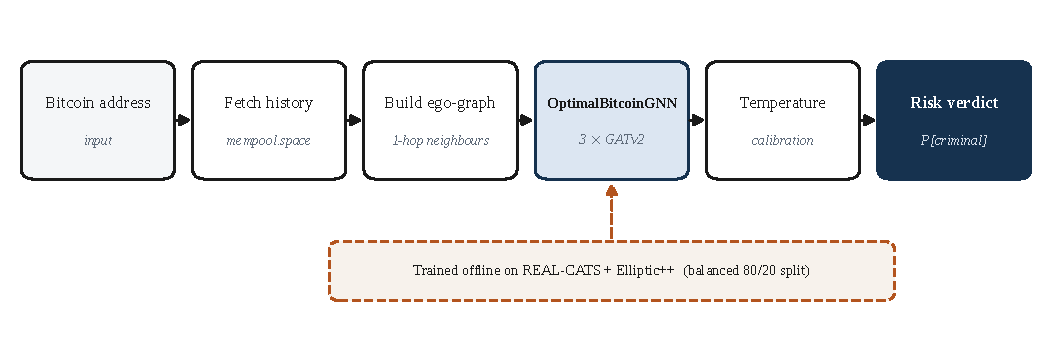
\includegraphics[width=0.98\linewidth]{figures/fig_method_overview.pdf}
\caption{End-to-end method. A Bitcoin address is expanded into a one-hop ego-graph from live
\texttt{mempool.space} data, passed through the trained GATv2 model, and returned as a
calibrated risk verdict. The same model is trained offline on the balanced merge of REAL-CATS
and Elliptic++.}
\label{fig:workflow}
\end{figure}

\section{Main Findings}
On a held-out test set of 21{,}718 wallets, the GNN reaches F\textsubscript{1}~$=0.869$ and
ROC-AUC~$=0.959$, clearly ahead of XGBoost (F\textsubscript{1}~$=0.755$) and the plain GCN
(F\textsubscript{1}~$=0.582$). The two controlled contrasts localise \emph{why}: the jump over
the plain GCN shows that per-transaction detail (amount, direction, timing) matters, and the
jump over XGBoost shows that the one-hop neighbourhood adds information beyond the wallet's
own statistics. After temperature scaling the probabilities are well calibrated, so the risk
score shown to a user can be read at face value.

\section{Document Structure}
Chapter~\ref{ch:goals} states the project goals. Chapter~\ref{ch:lit} reviews related work.
Chapter~\ref{ch:data} describes the two datasets and the unified feature schema.
Chapter~\ref{ch:eda} covers exploratory analysis and pre-processing. Chapter~\ref{ch:models}
details the data split, the ego-graph construction, and the three models.
Chapter~\ref{ch:experiments} defines the experimental protocol and metrics.
Chapter~\ref{ch:results} presents results and visualisations. Chapter~\ref{ch:summary}
concludes with limitations and future work. Appendices cover the deployed system's
characterisation and testing, and full reproducibility details.

% ===================== 2. GOALS ====================================
\chapter{Project Goals}\label{ch:goals}
The project has one primary goal and several concrete objectives that make it measurable.

\vspace{2pt}
\noindent\textbf{Primary goal.} Given a Bitcoin wallet address and its public transaction
history, automatically classify the wallet as \emph{criminal} or \emph{benign} and return a
calibrated risk score.

\begin{description}[leftmargin=1.3em,style=nextline,itemsep=3pt]
  \item[G1 --- Graph model.] Build a GNN that classifies a wallet from a one-hop ego-graph
    combining the wallet's behaviour with its transaction neighbourhood.
  \item[G2 --- Unified, balanced corpus.] Merge REAL-CATS and Elliptic++ onto a common
    feature schema, remove overlap and label conflicts, and produce a class-balanced,
    source-stratified train/test split.
  \item[G3 --- Cross-dataset generalisation.] Test whether one model trained across both
    sources generalises across crime types and time periods, rather than over-fitting one source.
  \item[G4 --- Rigorous evaluation.] Quantify performance against a tabular baseline (XGBoost)
    and a graph baseline (plain GCN) on identical wallets, using discrimination, per-class, and
    calibration metrics.
  \item[G5 --- Usable, calibrated product.] Serve the model as a live web application whose
    displayed confidence values are trustworthy (post-hoc calibration).
\end{description}

% ===================== 3. LITERATURE REVIEW ========================
\chapter{Literature Review}\label{ch:lit}
Cryptocurrency forensics has moved from heuristic rules to deep learning, and because
blockchain data is naturally a graph of wallets and transactions, GNNs have become the
dominant methodology. This review focuses on the strands most relevant to our design:
node/transaction-level GNNs, structural and subgraph analysis, temporal and imbalance-aware
methods, and the datasets that anchor the field.

\section{GNNs for Fraud Detection}
The foundational approach classifies individual wallets or transactions in isolation.
\citet{asiri2025gcn} show that optimised GCNs reach high accuracy on the Elliptic dataset when
structural features are combined with cost-sensitive training, validating GCN as a strong
baseline. \citet{zhang2024gatresnet} introduce GAT-ResNet, using graph \emph{attention} to
weigh the importance of neighbours and thereby handle noisy blockchain data better than plain
GCNs. This directly motivates our choice of a GATv2 attention backbone
\citep{brody2022gatv2,velickovic2018gat} over a vanilla GCN \citep{kipf2017gcn}.

\section{Structural and Subgraph Analysis}
Node-level models often miss sophisticated actors who launder through long chains of
intermediary wallets. \citet{ouyang2024subgraph} argue that laundering schemes such as
``peel chains'' appear as distinct geometric motifs in the graph rather than as isolated bad
nodes, and that analysing the surrounding subgraph captures operations that node-centric
models miss. This supports our decision to classify a wallet from its neighbourhood rather than
from its features alone.

\section{Temporal Behaviour and Class Imbalance}
Two operational hurdles are the temporal nature of the data and the scarcity of illicit labels.
\citet{alarab2022lstm} combine GCNs with an LSTM to model how transaction behaviour evolves
over time and address the cold-start problem via active learning. The RL-GNN fusion line of
work \citep{rlgnn2025} tackles real-time detection in imbalanced streams by dynamically
adjusting fraud thresholds to cope with concept drift. We do not model time recurrently, but we
adopt imbalance-aware practice by \emph{balancing} the training corpus and encoding a
normalised timestamp on every edge.

\section{Datasets and Benchmarking}
High-quality labelled data is the prerequisite for all of the above. The Elliptic dataset
\citep{weber2019elliptic} and its extension Elliptic++ \citep{ellipticpp2023} are the standard
benchmarks but focus on 2014--2017 theft/Ponzi activity. REAL-CATS \citep{realcats2024}
expands coverage into modern threats (scams, ransomware, extortion, darknet markets). Using
both is central to our generalisation hypothesis.

\section{Positioning of This Project}
Most reviewed studies train and test on a single source and therefore learn source-specific
patterns. Our contribution is to build a \emph{unified} model across Elliptic++ (theft/Ponzi) and
REAL-CATS (modern cybercrime), testing whether illicit activity carries a structural signature
robust across crime types and time periods --- a question the prior single-dataset work leaves
open.

% ===================== 4. DATA DESCRIPTION ==========================
\chapter{Data Description}\label{ch:data}

\section{Sources}
\textbf{REAL-CATS} \citep{realcats2024} is an expert-curated dataset of Bitcoin wallets linked
to criminal activity, compiled by domain analysts from public criminal-wallet reports
(sanctions lists, ransomware disclosures, law-enforcement notices), paired with a benign
control set. Its labels come from human reporting rather than on-chain inference; the material
was collected through roughly 2023--2024. \textbf{Elliptic++} \citep{ellipticpp2023} extends the
original Elliptic dataset \citep{weber2019elliptic}; its transactions span roughly 2014--2017,
organised into 49 time-steps of about two weeks each.

\section{Unified Feature Schema}
Both datasets are mapped onto a common schema of nineteen features computable from either
source: eleven shared base features (total transactions, total sent and received, total fees,
lifetime, send and receive counts, max/min sent and received), three features derivable from
both (mean blocks between transactions, mean fee share, average transaction size), and five
engineered features (send/receive ratio, activity rate, fee per transaction, transaction-size
range, in/out balance). Every feature is also stored as its $\log(1+x)$ transform. After
correlation pruning --- dropping seven features that were highly correlated with another
($r>0.95$) --- the model uses the twelve least-redundant log-scaled features listed in
Table~\ref{tab:features}.

\begin{table}[H]
\centering\small
\caption{The twelve log-scaled features used by the model (after correlation pruning).}
\label{tab:features}
\renewcommand{\arraystretch}{1.15}
\begin{tabularx}{\linewidth}{>{\ttfamily\footnotesize\raggedright\arraybackslash}p{5.6cm} >{\raggedright\arraybackslash}X}
\toprule
\normalfont\bfseries Feature & \textbf{Meaning} \\
\midrule
fee\_per\_tx\_log          & Average fee paid per transaction \\
fee\_share\_mean\_log      & Mean fraction of transaction value spent on fees \\
tx\_size\_range\_log       & Spread between largest and smallest sent amount \\
total\_txs\_log            & Lifetime number of transactions \\
send\_receive\_ratio\_log  & Ratio of outgoing to incoming activity \\
avg\_tx\_size\_log         & Average sent amount \\
max\_sent\_log             & Largest single amount sent \\
in\_out\_balance\_log      & Balance between received and sent volume \\
max\_received\_log         & Largest single amount received \\
blocks\_btwn\_txs\_mean\_log & Mean number of blocks between transactions \\
activity\_rate\_log        & Transactions per unit lifetime \\
lifetime\_seconds\_log     & Time between first and last transaction \\
\bottomrule
\end{tabularx}
\end{table}

\section{Balanced Split}
A balancing step drops cross-source addresses whose labels disagree, collapses agreeing
duplicates, keeps every criminal wallet plus a matched random sample of benign wallets within
each source, and produces a stratified 80/20 split keyed on the joint (label, source). Both
classes and both sources appear in identical proportions in train and test (Table~\ref{tab:split});
the random seed is fixed throughout.

\begin{table}[H]
\centering\small
\caption{Balanced, source-stratified train/test split.}
\label{tab:split}
\begin{tabular}{lrrrrr}
\toprule
\textbf{Split} & \textbf{Rows} & \textbf{Criminal} & \textbf{Benign} & \textbf{REAL-CATS} & \textbf{Elliptic++} \\
\midrule
Training set & 86{,}870 & 43{,}435 & 43{,}435 & 64{,}044 & 22{,}826 \\
Test set     & 21{,}718 & 10{,}859 & 10{,}859 & 16{,}012 &  5{,}706 \\
\bottomrule
\end{tabular}
\end{table}

% ===================== 5. EDA & PREPROCESSING =======================
\chapter{Data Exploration and Pre-processing}\label{ch:eda}

\section{Exploratory Analysis}
Exploratory analysis of both datasets guided every downstream choice. In \textbf{Elliptic++},
labels are heavily imbalanced (illicit transactions average $\sim$11\% and only a small
fraction of wallets are labelled), and illicit nodes are typically low-degree while licit nodes
form high-degree hubs --- illicit actors rarely form tightly connected clusters and instead
blend into the wider network by transacting with unknown or licit nodes. Value distributions
differ by class: illicit transactions concentrate at lower values with a sharper peak, whereas
licit transactions have a heavier right tail. In \textbf{REAL-CATS}, criminal wallets are more
active than benign ones (median transaction count $4$ vs.\ $2$) and move more money
(median total sent \$2{,}426 vs.\ \$1{,}049), which confirms that activity- and
volume-based features are discriminative. The criminal category mix is dominated by scams
and ransomware, with darknet markets and mixing services rarer but showing the highest
transaction intensity.

\section{Pre-processing Pipeline}
The findings above translate into a fixed pre-processing pipeline, applied identically at
training and at inference:
\begin{enumerate}[leftmargin=1.4em,itemsep=2pt]
  \item \textbf{Cleaning.} Remove zero-transaction addresses; resolve satoshi-to-BTC unit
    scaling so amounts are on a consistent scale.
  \item \textbf{Feature engineering.} Compute the nineteen-feature schema, including the five
    engineered ratios, from raw transaction records.
  \item \textbf{Log transform.} Apply $\log(1+x)$ to every feature to compress heavy tails
    seen in the EDA.
  \item \textbf{Clipping.} Clip engineered features to training-derived ranges (activity rate
    to $[0,1000]$; send/receive ratio and in/out balance to $[0,100]$; fee share to $[0,1]$) so
    a live wallet cannot produce out-of-distribution values.
  \item \textbf{Correlation pruning.} Drop the seven features with pairwise $r>0.95$, leaving
    the twelve features of Table~\ref{tab:features}.
  \item \textbf{Balancing \& split.} Balance classes within each source and take the stratified
    80/20 split of Table~\ref{tab:split}.
\end{enumerate}
Maintaining \emph{train/inference parity} --- running exactly this pipeline on live wallet data ---
was essential: an early unit mismatch (satoshis vs.\ BTC) made inference features up to
$90{,}000\times$ larger than training features and skewed predictions until the scaling and
clipping were made identical on both sides.

% ===================== 6. MODELS ===================================
\chapter{Data Split, Ego-Graphs, and Models}\label{ch:models}

\section{Per-Wallet Ego-Graphs}
For each wallet a small graph is built. The wallet sits at the centre carrying the twelve log
features. Every counter-party it has transacted with appears as a \emph{ghost} node; at
forward time the model replaces each ghost's zero-feature placeholder with a learned
embedding plus a node-type embedding, so ghost neighbours are not treated as fresh wallets
with all-zero behaviour. Each interaction is a directed edge with three features: the log of the
amount transferred, a direction flag (1 outgoing, 0 incoming), and a timestamp normalised
against the Bitcoin genesis block. Transaction history is fetched from the public
\texttt{mempool.space} API and cached per address.

\section{The Model: OptimalBitcoinGNN}
The main model is a three-layer GATv2 graph attention network
\citep{brody2022gatv2,fey2019pyg} with $4\!\to\!4\!\to\!2$ attention heads, hidden size 64, and
an edge dimension of 3. It uses residual connections from the input through the GNN layers,
DropEdge regularisation \citep{rong2020dropedge}, and a hybrid readout that concatenates the
centre-node embedding with global mean-pool and global max-pool
($3\times 64 = 192$), followed by a $192\!\to\!64\!\to\!2$ classifier. Figure~\ref{fig:arch}
shows the architecture.

\begin{figure}[H]
\centering
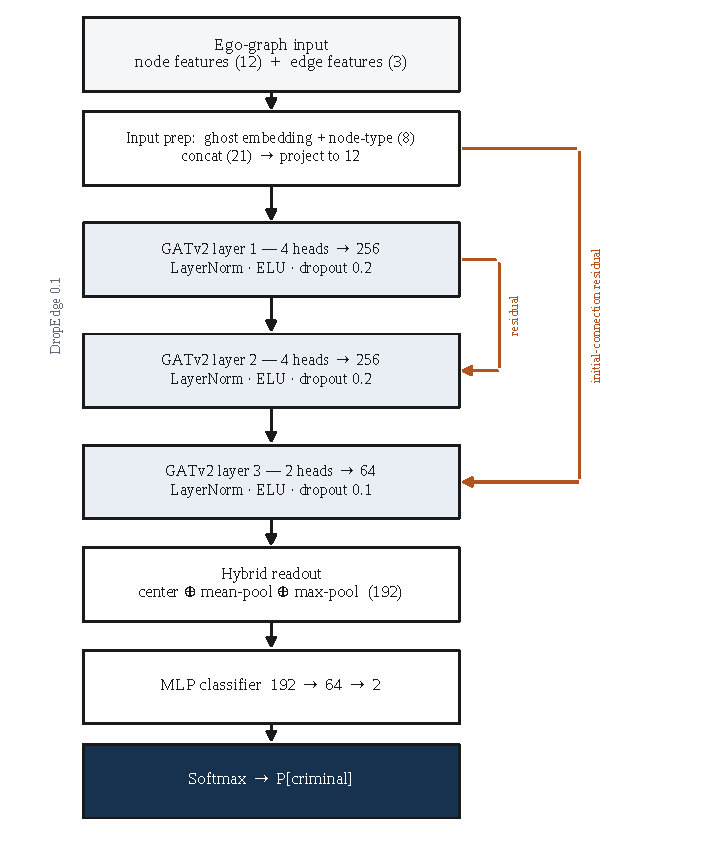
\includegraphics[width=0.52\linewidth]{figures/fig_architecture.pdf}
\caption{OptimalBitcoinGNN architecture: three GATv2 layers with multi-head attention, learnable
ghost/node-type embeddings, an initial-connection residual, and a hybrid
(centre~$\oplus$~mean-pool~$\oplus$~max-pool) readout feeding a two-layer classifier.}
\label{fig:arch}
\end{figure}

\section{Baselines}
Two baselines each remove exactly one ingredient, so the comparisons are controlled:
\begin{itemize}[leftmargin=1.4em,itemsep=2pt]
  \item \textbf{XGBoost (tabular)} \citep{chen2016xgboost}: trained on the same twelve features
    and the same split, but with \emph{no} graph. The contrast with the GNN isolates the value
    of the one-hop neighbourhood.
  \item \textbf{Basic GCN (graph)} \citep{kipf2017gcn}: a vanilla GCN on the same ego-graphs
    but without learnable ghost embeddings, without the input-to-final residual, and with a plain
    mean-pool readout instead of the hybrid readout. The contrast isolates the value of our
    architectural additions and of per-edge transaction detail.
\end{itemize}

\section{Calibration}
Neural classifiers are often over-confident \citep{guo2017calibration}. After training, a single
temperature parameter is fit by LBFGS on a held-out calibration slice and applied at inference
in the backend, so the displayed probabilities can be read as honest
confidence values.

% ===================== 7. EXPERIMENTS ==============================
\chapter{Experiments}\label{ch:experiments}

\section{Protocol}
The 80/20 stratified split gives the canonical train and test sets. Inside training, the training
pool is further split 85/15 (fixed seed) into train and validation, the latter used for early
stopping and best-epoch selection on validation F\textsubscript{1}. A small slice is reserved
\emph{before} that split, exclusively for temperature scaling. All three models are trained and
evaluated on \emph{exactly the same wallets} --- the rows whose address has a cached
ego-graph --- so the comparison is row-for-row fair; XGBoost is retrained on the same
intersection rather than on the full CSV.

\section{Measurement Method and Metrics}
The primary metric is F\textsubscript{1} on the held-out test split, complemented by a standard
battery so a single number cannot hide the full picture (Table~\ref{tab:metricfamilies}). Model
selection during training uses validation F\textsubscript{1} with early stopping (patience 20).
The evaluation step also dumps misclassified test addresses (false positives and false
negatives) to CSV and writes per-feature gradient-saliency scores to JSON.

\begin{table}[H]
\centering\small
\caption{Evaluation metrics.}
\label{tab:metricfamilies}
\begin{tabularx}{\linewidth}{l Y}
\toprule
\textbf{Family} & \textbf{Metrics} \\
\midrule
Discrimination & Accuracy, Precision, Recall, F\textsubscript{1}, ROC-AUC, PR-AUC \\
Per-class      & Precision / Recall / F\textsubscript{1} for the benign and criminal classes \\
Confusion      & Confusion matrix on the test set \\
Calibration    & Brier score, Expected Calibration Error, reliability diagram \\
\bottomrule
\end{tabularx}
\end{table}

\section{Key Hyperparameters}
Table~\ref{tab:hparams} lists the settings that reproduce the reported numbers; the full set is
in Appendix~\ref{app:repro}.

\begin{table}[H]
\centering\small
\caption{Key hyperparameters.}
\label{tab:hparams}
\begin{tabularx}{\linewidth}{l Y}
\toprule
\textbf{Component} & \textbf{Setting} \\
\midrule
GNN         & $3\times$ GATv2Conv (4/4/2 heads), hidden 64, edge dim 3, dropout 0.2 (final 0.3), DropEdge 0.1 \\
Readout     & centre $\oplus$ mean-pool $\oplus$ max-pool ($192$), classifier $192\!\to\!64\!\to\!2$ \\
Optimiser   & AdamW, lr $10^{-3}$, weight decay $0.01$, grad-clip $1.0$ \\
Scheduler   & OneCycleLR, max lr $5\times10^{-3}$, pct-start $0.1$ \\
Loss        & Cross-entropy, label smoothing $0$ \\
Schedule    & $\le 150$ epochs, batch 64, early stop on val F\textsubscript{1} (patience 20) \\
Calibration & LBFGS, max-iter 50, lr $0.01$ \\
XGBoost     & 200 estimators, max-depth 8, lr 0.1, subsample 0.8, colsample 0.8 \\
Basic GCN   & $3\times$ GCNConv, hidden 64, mean-pool readout, dropout 0.2 \\
Seed        & 42 (split, sub-split, dataloader, torch RNG) \\
\bottomrule
\end{tabularx}
\end{table}

% ===================== 8. RESULTS ==================================
\chapter{Results and Conclusions}\label{ch:results}

\section{Head-to-Head Comparison}
Table~\ref{tab:results} and Figure~\ref{fig:baseline} report all three models on the same
11{,}880 shared test wallets. The GNN leads on every metric except precision, where it is within
half a point of XGBoost while recovering \emph{far} more criminals (recall 0.884 vs.\ 0.673).

\begin{table}[H]
\centering\small
\caption{Test-set performance on identical wallets (n\,=\,11{,}880 shared). Best per column in bold.}
\label{tab:results}
\begin{tabular}{lccccc}
\toprule
\textbf{Model} & \textbf{F\textsubscript{1}} & \textbf{Accuracy} & \textbf{Precision} & \textbf{Recall} & \textbf{ROC-AUC} \\
\midrule
OptimalGNN (ours)          & \textbf{0.869} & \textbf{0.894} & 0.855 & \textbf{0.884} & \textbf{0.959} \\
XGBoost (tabular)          & 0.755 & 0.826 & \textbf{0.861} & 0.673 & 0.909 \\
Basic GCN (graph baseline) & 0.582 & 0.701 & 0.658 & 0.522 & 0.777 \\
\bottomrule
\end{tabular}
\end{table}

\begin{figure}[H]
\centering
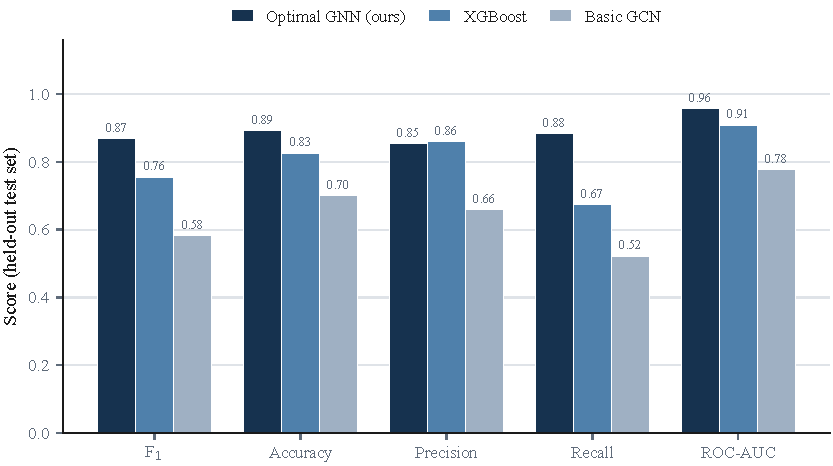
\includegraphics[width=0.72\linewidth]{figures/fig_metric_comparison.pdf}
\caption{Metric-by-metric comparison of the three models on the shared held-out test set.}
\label{fig:baseline}
\end{figure}

\section{Training Dynamics}
The GNN was trained for up to 150 epochs with early stopping on the validation F\textsubscript{1}.
Figure~\ref{fig:training} shows training loss falling smoothly while validation F\textsubscript{1}
plateaus; the best epoch (81) is selected and the remaining epochs add no validation gain,
confirming the model is neither under- nor over-trained.

\begin{figure}[H]
\centering
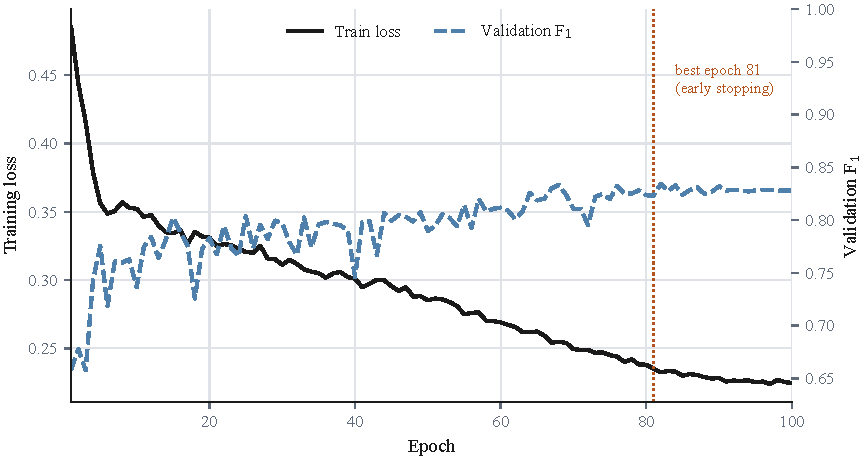
\includegraphics[width=0.72\linewidth]{figures/fig_training_curves.pdf}
\caption{Training loss (left axis) and validation F\textsubscript{1} (right axis) over epochs.
The dotted line marks the early-stopping / best epoch.}
\label{fig:training}
\end{figure}

\section{What the Gaps Mean}
Two contrasts tell the story. \textbf{Basic GCN $\rightarrow$ OptimalGNN} ($+0.29$
F\textsubscript{1}): per-transaction detail (amount, direction, timing) plus our architectural
additions matter a great deal. \textbf{XGBoost $\rightarrow$ OptimalGNN} ($+0.11$
F\textsubscript{1}, $+0.21$ recall): the one-hop neighbourhood carries information the wallet's
own statistics do not capture --- the project's central result, and evidence for a structural
signature of illicit activity that holds across the two merged datasets.

\section{Discrimination and Errors}
The confusion matrices (Figure~\ref{fig:cm}) contrast all three models on the same wallets.
Our GNN shows a balanced error profile --- 553 false negatives and 713 false positives out of
11{,}880 --- missing relatively few criminals while keeping benign wallets mostly clear, whereas
the plain GCN misses almost half of the criminal class. The ROC curves (Figure~\ref{fig:roc})
give the GNN AUC~$=0.959$, well above XGBoost ($0.909$) and the plain GCN ($0.777$).

\begin{figure}[H]
\centering
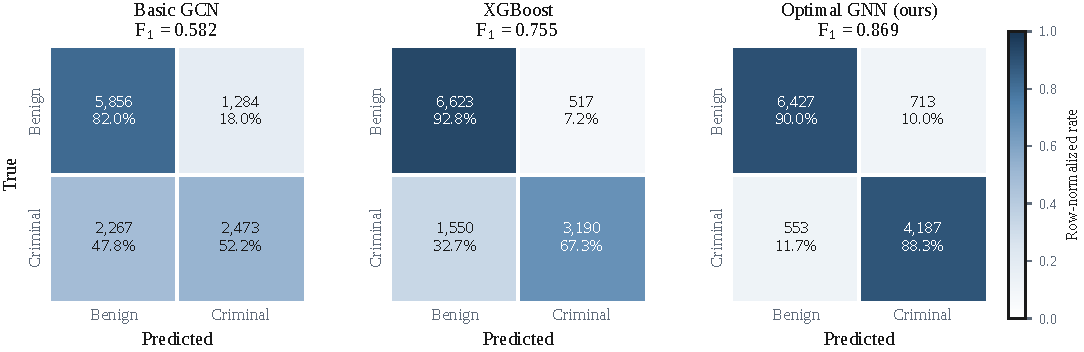
\includegraphics[width=0.9\linewidth]{figures/fig_confusion_panel.pdf}
\caption{Confusion matrices on the shared held-out test set (colour is row-normalized; cells show
counts and row percentages). Left to right: Basic GCN, XGBoost, and our Optimal GNN.}
\label{fig:cm}
\end{figure}

\begin{figure}[H]
\centering
\IfFileExists{figures/fig_roc.pdf}
  {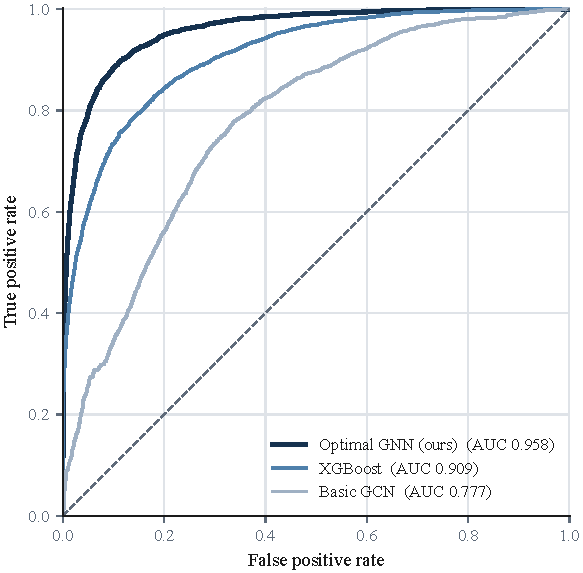
\includegraphics[width=0.56\linewidth]{figures/fig_roc.pdf}}
  {\fbox{\parbox{0.8\linewidth}{\centering\small\vspace{2em}\textit{fig\_roc.pdf} ---
   generate with \texttt{python report/figure\_scripts/make\_figures.py} inside the project
   venv (re-scores the cached test graphs), then recompile.\vspace{2em}}}}
\caption{ROC curves for the three models on the held-out test set.}
\label{fig:roc}
\end{figure}

\section{Calibration}
After temperature scaling ($T=1.06$), the predicted probabilities are usable as risk thresholds.
The reliability diagram (Figure~\ref{fig:reliability}) tracks the diagonal closely, with a low
Expected Calibration Error, so the risk score the web application displays can be trusted at face
value rather than read only as a ranking.

\begin{figure}[H]
\centering
\IfFileExists{figures/fig_reliability.pdf}
  {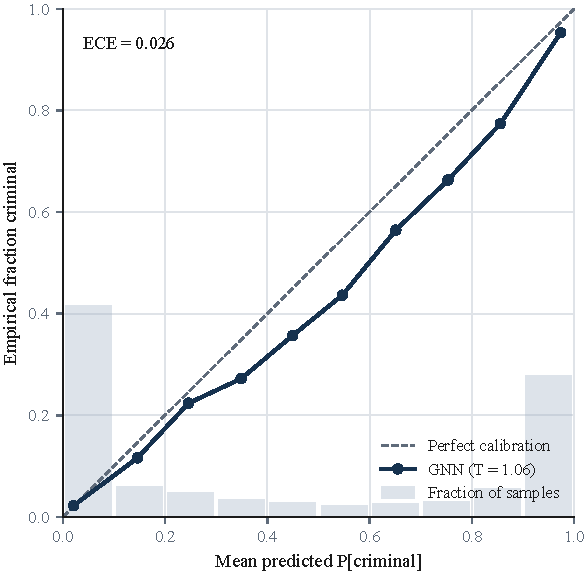
\includegraphics[width=0.56\linewidth]{figures/fig_reliability.pdf}}
  {\fbox{\parbox{0.8\linewidth}{\centering\small\vspace{2em}\textit{fig\_reliability.pdf} ---
   generate with \texttt{python report/figure\_scripts/make\_figures.py} inside the project
   venv (re-scores the cached test graphs), then recompile.\vspace{2em}}}}
\caption{Reliability diagram for the GNN after temperature scaling; bars show the fraction of
test samples in each confidence bin.}
\label{fig:reliability}
\end{figure}

\section{Interpretability}
Gradient-saliency over the twelve inputs (Figure~\ref{fig:fi}) is dominated by fee behaviour:
\texttt{fee\_per\_tx} ($0.63$) and \texttt{fee\_share\_mean} ($0.18$) together account for the
majority of attributed importance, with transaction-size range and total transactions next. This
matches the EDA intuition that \emph{how} a wallet spends on fees and structures its
transactions, more than raw volume, separates criminal from benign behaviour.

\begin{figure}[H]
\centering
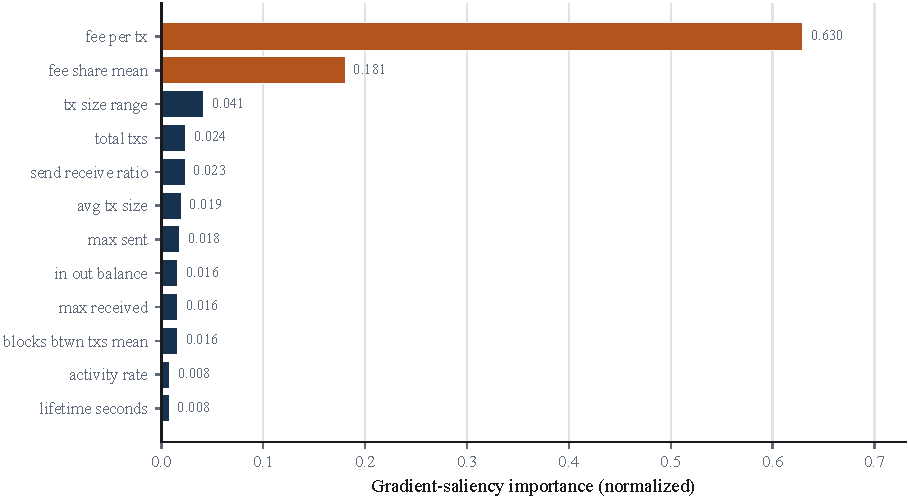
\includegraphics[width=0.72\linewidth]{figures/fig_feature_importance.pdf}
\caption{Per-feature gradient-saliency importance for the GNN (twelve log-scaled features).}
\label{fig:fi}
\end{figure}

% ===================== 9. SUMMARY ==================================
\chapter{Summary and Future Work}\label{ch:summary}

\section{Summary}
We built a graph-based Bitcoin wallet risk classifier that decides, from a single address and
its public history, whether a wallet has been used for criminal activity. Trained on a balanced
merge of REAL-CATS and Elliptic++, a three-layer GATv2 network reaches F\textsubscript{1}
$=0.869$ and ROC-AUC $=0.959$ on a held-out test set, beating a tabular XGBoost baseline by
$\sim$11 F\textsubscript{1} points and a plain GCN by $\sim$29. The controlled baselines show
the gain comes specifically from reading the wallet's transaction neighbourhood, supporting the
hypothesis that illicit activity has a structural signature that generalises across crime types and
time periods. The model is deployed as a calibrated, live web application (\live).

\section{Challenges}
The main challenges were data-engineering rather than modelling: enforcing train/inference
parity after a satoshi/BTC unit mismatch, keeping the probability range from collapsing (fixed by
learnable ghost embeddings and by removing label smoothing, then temperature scaling), and
building tens of thousands of ego-graphs against a rate-limited public API.

\section{Future Work}
Natural extensions are: (i) rebuild the training ego-graphs at full transaction pagination (current
cached graphs captured only the first 25 transactions per wallet, a structure mismatch versus the
500-transaction inference path); (ii) train on the larger graph corpus once the full download
completes; (iii) add an independent validation split for calibration instead of reusing the test
set; (iv) build a live adversarial test set of recent wallets in neither source to stress-test
generalisation via precision@$k$; and (v) explore temporal GNN extensions and focal loss (already
implemented but unused) for the residual class-hard cases.

% ===================== BIBLIOGRAPHY ================================
\bibliographystyle{plainnat}
\bibliography{references}

% ===================== APPENDICES ==================================
\appendix
\chapter{Deployed System: Characterisation and Testing}\label{app:system}
A web application was built to \emph{use} the model, so per the course guidelines it is
characterised and tested here rather than in the main body.

\section{Architecture}
The system has two components. A \textbf{FastAPI} backend loads the trained weights
(\texttt{outputs/gnn\_model.pt}) and the temperature scaler, exposes an \texttt{/analyze}
endpoint that, given an address, fetches its transactions from \texttt{mempool.space}, builds
the ego-graph, runs inference, and returns a calibrated verdict plus supporting data. A
\textbf{React\,+\,Vite} frontend lets a visitor paste an address and see the verdict, an
explanation, and transaction context. The app is deployed on the BGU CS department servers at
\live.

\section{Functional Requirements}
The user pastes a valid Bitcoin address; the system returns a criminal/benign verdict with a
calibrated probability, the top contributing features, and a summary of the wallet's transaction
history and balance. Invalid or empty addresses are rejected with a clear message.

\section{Non-Functional Requirements}
Analysis runs off the event loop so the UI stays responsive; wallet data is cached to avoid
repeated API calls; transaction fetching is paginated to 500 transactions and issued
sequentially to respect \texttt{mempool.space} rate limits; the UI meets basic accessibility and
contrast guidelines (verdict shown above model internals).

\section{Testing}
Testing focused on model quality and behaviour (Chapters~\ref{ch:experiments}--\ref{ch:results}):
held-out evaluation of all three models on identical wallets; calibration checks (Brier, ECE,
reliability); per-source slicing to confirm neither REAL-CATS nor Elliptic++ carries the headline
number alone; a misclassification dump (false positives / false negatives to CSV); and
gradient-saliency interpretability. A planned extension is an automated unit-test suite and a live
adversarial precision@$k$ set. Every evaluation artifact regenerates from the saved weights and
the calibration scalar (seed 42).

\section{Reproducibility}\label{app:repro}
\textbf{Repository.}~\repo. \textbf{Live demo.}~\live.

\vspace{4pt}
\noindent Run the full offline pipeline with:
\begin{quote}\ttfamily
python run\_pipeline.py --all
\end{quote}
or step by step: \texttt{--prepare} (build the balanced dataset) $\rightarrow$ \texttt{--graphs}
(build/cache ego-graphs) $\rightarrow$ \texttt{--baseline} (XGBoost) $\rightarrow$ \texttt{--train}
(GNN) $\rightarrow$ \texttt{--evaluate} (metrics, comparison, calibration, error dumps). A single
seed (42) governs the dataset split, the validation sub-split, the dataloader shuffle, and the
torch RNG, so every number in this report is reproducible from the saved model weights and the
temperature scalar. Stack: PyTorch + PyTorch Geometric, XGBoost, FastAPI, React + Vite, and the
\texttt{mempool.space} API.

\end{document}
